
\documentclass[12pt]{article}
\usepackage[utf8]{inputenc}
\usepackage{amsmath,amsfonts}
\usepackage{graphicx}
\usepackage{hyperref}
\usepackage{booktabs}
\usepackage{geometry}
\usepackage{caption}
\usepackage{float}
\usepackage{fancyhdr}
\usepackage{enumitem}
\usepackage{url}
\geometry{margin=1in}

\title{Binary Classification of Diabetes using a Manually Implemented Multilayer Perceptron}
\author{Hiba Amenhar \\ Master Student – IAA \\ Academic Year 2024–2025}
\date{}

\pagestyle{fancy}
\fancyhf{}
\rhead{Binary Diabetes Classification}
\lhead{Hiba Amenhar}
\rfoot{\thepage}

\begin{document}

\maketitle

\begin{abstract}
This paper presents a comprehensive implementation and analysis of a Multilayer Perceptron (MLP) for binary classification on the Pima Indians Diabetes dataset. Without relying on machine learning frameworks, we coded a neural network from scratch using NumPy. The model is trained using stochastic gradient descent (SGD) and evaluated through standard classification metrics. We examine the network’s design, mathematical foundation, training process, performance outcomes, and avenues for future improvements.
\end{abstract}

\textbf{Keywords:} Diabetes, Multilayer Perceptron, Classification, Neural Networks, Python, Machine Learning, SGD

\tableofcontents
\newpage

\section{Introduction}
Diabetes mellitus is one of the most prevalent chronic diseases worldwide, with significant health and economic impacts. The need for early detection is vital to prevent complications. With the rise of artificial intelligence, machine learning models are increasingly being applied to medical data for predictive diagnostics. This paper explores the implementation of a neural network classifier developed from scratch using only NumPy to identify diabetic patients from the Pima Indians dataset.

\section{Background and Related Work}
Machine learning methods like decision trees, logistic regression, support vector machines, and neural networks have all been applied to the diabetes dataset. Deep learning models, particularly MLPs, have shown promise due to their capacity to capture complex nonlinear patterns. However, many implementations rely on libraries such as TensorFlow or PyTorch. In contrast, this project implements an MLP manually, to better understand its mechanics and limitations.

\section{Dataset Description}
The Pima Indians Diabetes dataset includes 768 female patients aged 21 and above from the Pima Indian heritage. Each instance consists of 8 features:
\begin{itemize}
    \item \textbf{Pregnancies}
    \item \textbf{Glucose}
    \item \textbf{BloodPressure}
    \item \textbf{SkinThickness}
    \item \textbf{Insulin}
    \item \textbf{BMI}
    \item \textbf{DiabetesPedigreeFunction}
    \item \textbf{Age}
\end{itemize}
The target variable is \textbf{Outcome} (1 if diabetic, 0 otherwise).

\section{Methodology}
\subsection{Data Preprocessing}
Several features contain zero values, which are medically invalid. These are replaced with the median of each feature. The data is then standardized using z-score normalization. We split the dataset into 80\% training and 20\% testing using stratified sampling.

\subsection{Model Architecture}
The MLP is composed of:
\begin{itemize}
    \item Input layer: 8 neurons (for 8 features)
    \item Hidden layers: two layers with 16 and 8 neurons respectively
    \item Output layer: 1 neuron with sigmoid activation
\end{itemize}

\subsection{Mathematical Formulation}
Forward propagation:
\[
Z^{[l]} = A^{[l-1]}W^{[l]} + b^{[l]}
\]
\[
A^{[l]} = \text{ReLU}(Z^{[l]}), \quad A^{[L]} = \sigma(Z^{[L]})
\]

Loss function (Binary Cross-Entropy):
\[
J = -\frac{1}{m} \sum_{i=1}^{m} \left[y_i \log(\hat{y}_i) + (1 - y_i) \log(1 - \hat{y}_i)\right]
\]

Backward propagation:
\[
dZ^{[L]} = A^{[L]} - Y
\]
\[
dW^{[l]} = \frac{1}{m} A^{[l-1]T} dZ^{[l]}, \quad db^{[l]} = \frac{1}{m} \sum dZ^{[l]}
\]

\subsection{Training Procedure}
Training was performed using mini-batch SGD with:
\begin{itemize}
    \item Epochs: 100
    \item Batch size: 32
    \item Learning rate: 0.01
\end{itemize}
We shuffle the data at each epoch and compute forward and backward passes to update the weights.

\section{Results}
\subsection{Evaluation Metrics}
The model performance is evaluated using:
\begin{itemize}
    \item Accuracy
    \item Precision, Recall
    \item F1-score
    \item Confusion Matrix
\end{itemize}

\subsection{Performance Summary}
\begin{itemize}
    \item Accuracy: 65\%
    \item Precision: 0.65 (Class 0), 0.00 (Class 1)
    \item Recall: 1.00 (Class 0), 0.00 (Class 1)
    \item F1-score: 0.79 (Class 0), 0.00 (Class 1)
\end{itemize}

\subsection{Visualizations}
\begin{figure}[H]
\centering
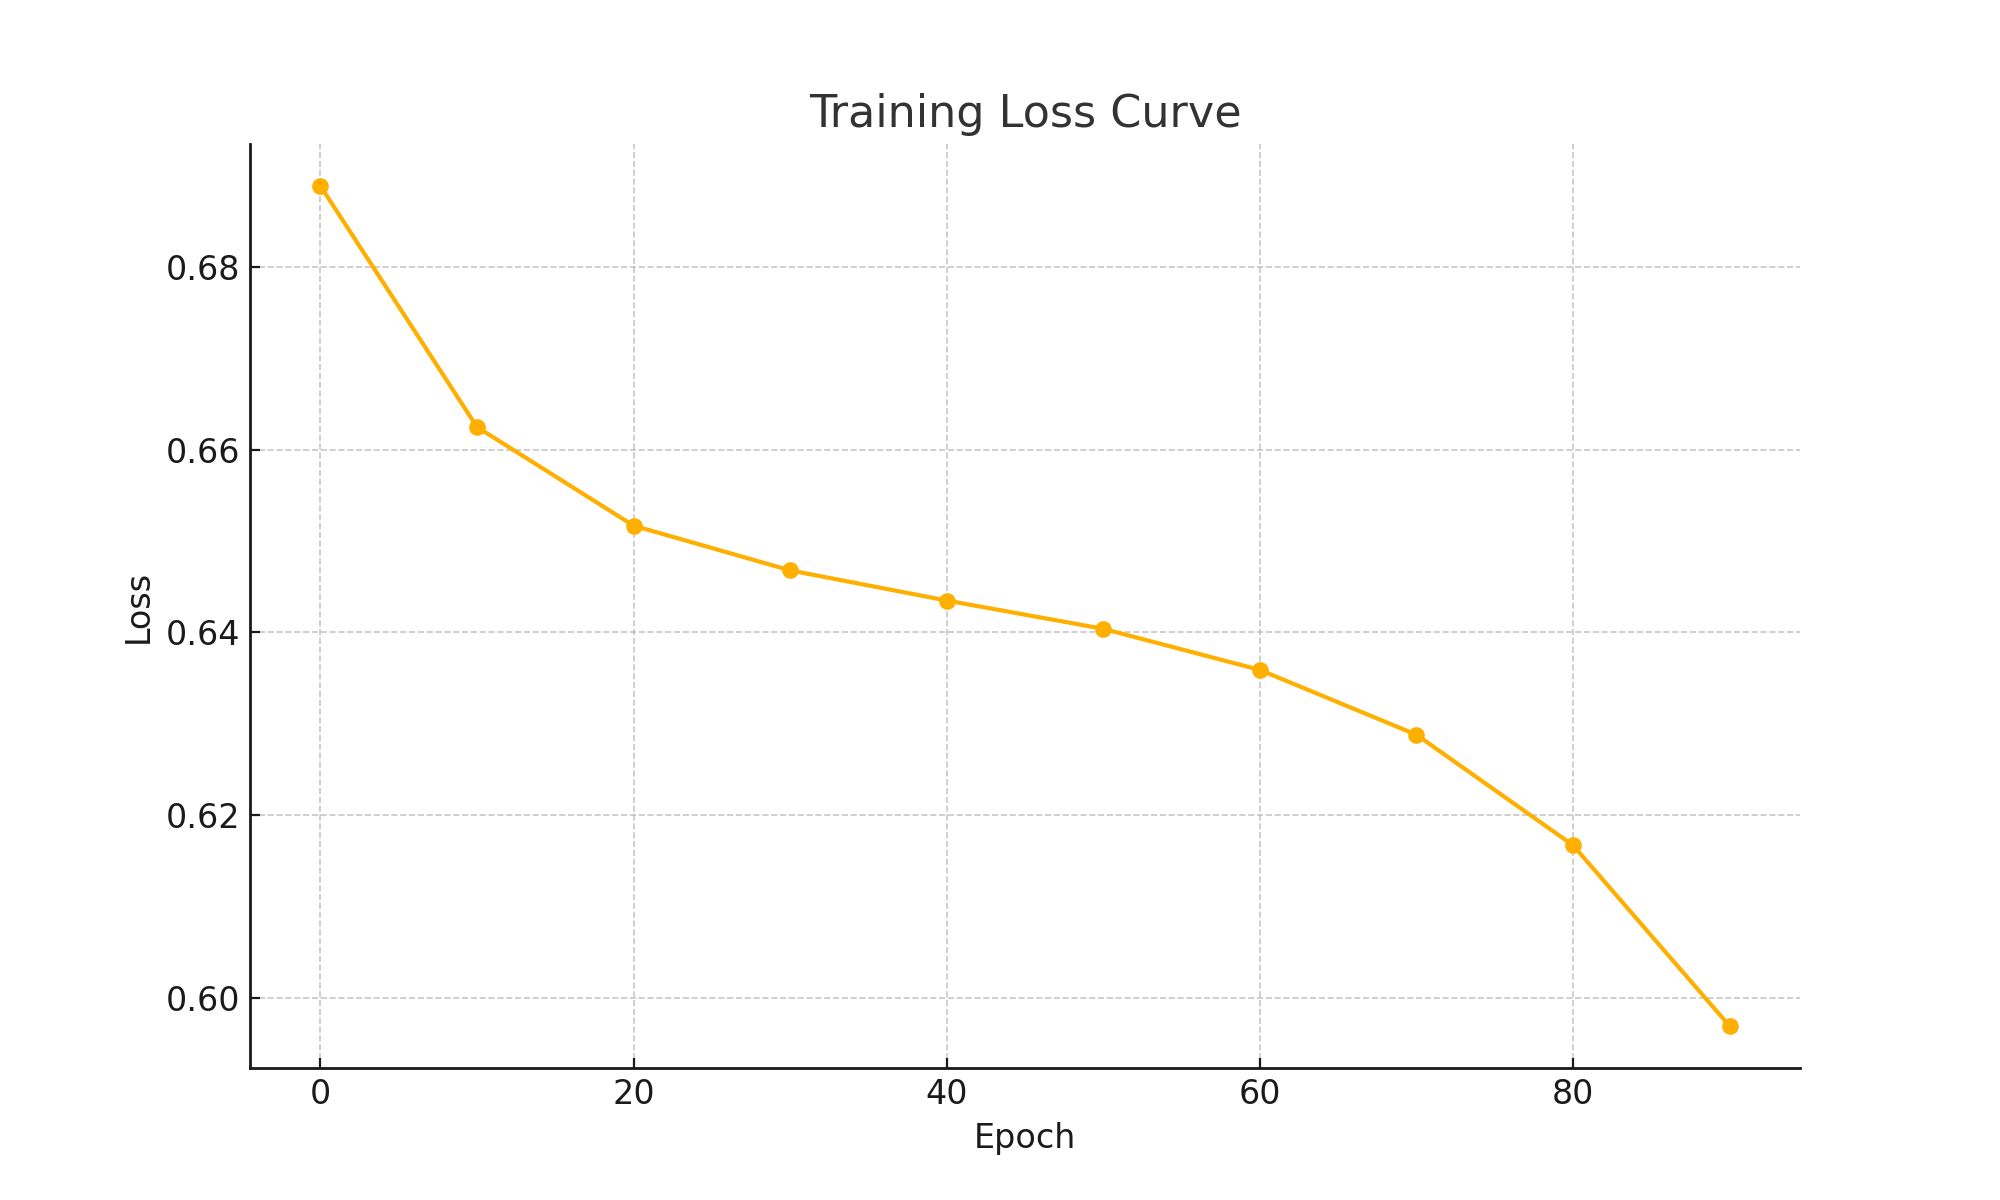
\includegraphics[width=0.85\linewidth]{loss_curve.png}
\caption{Training Loss Curve over 100 epochs}
\end{figure}

\begin{figure}[H]
\centering
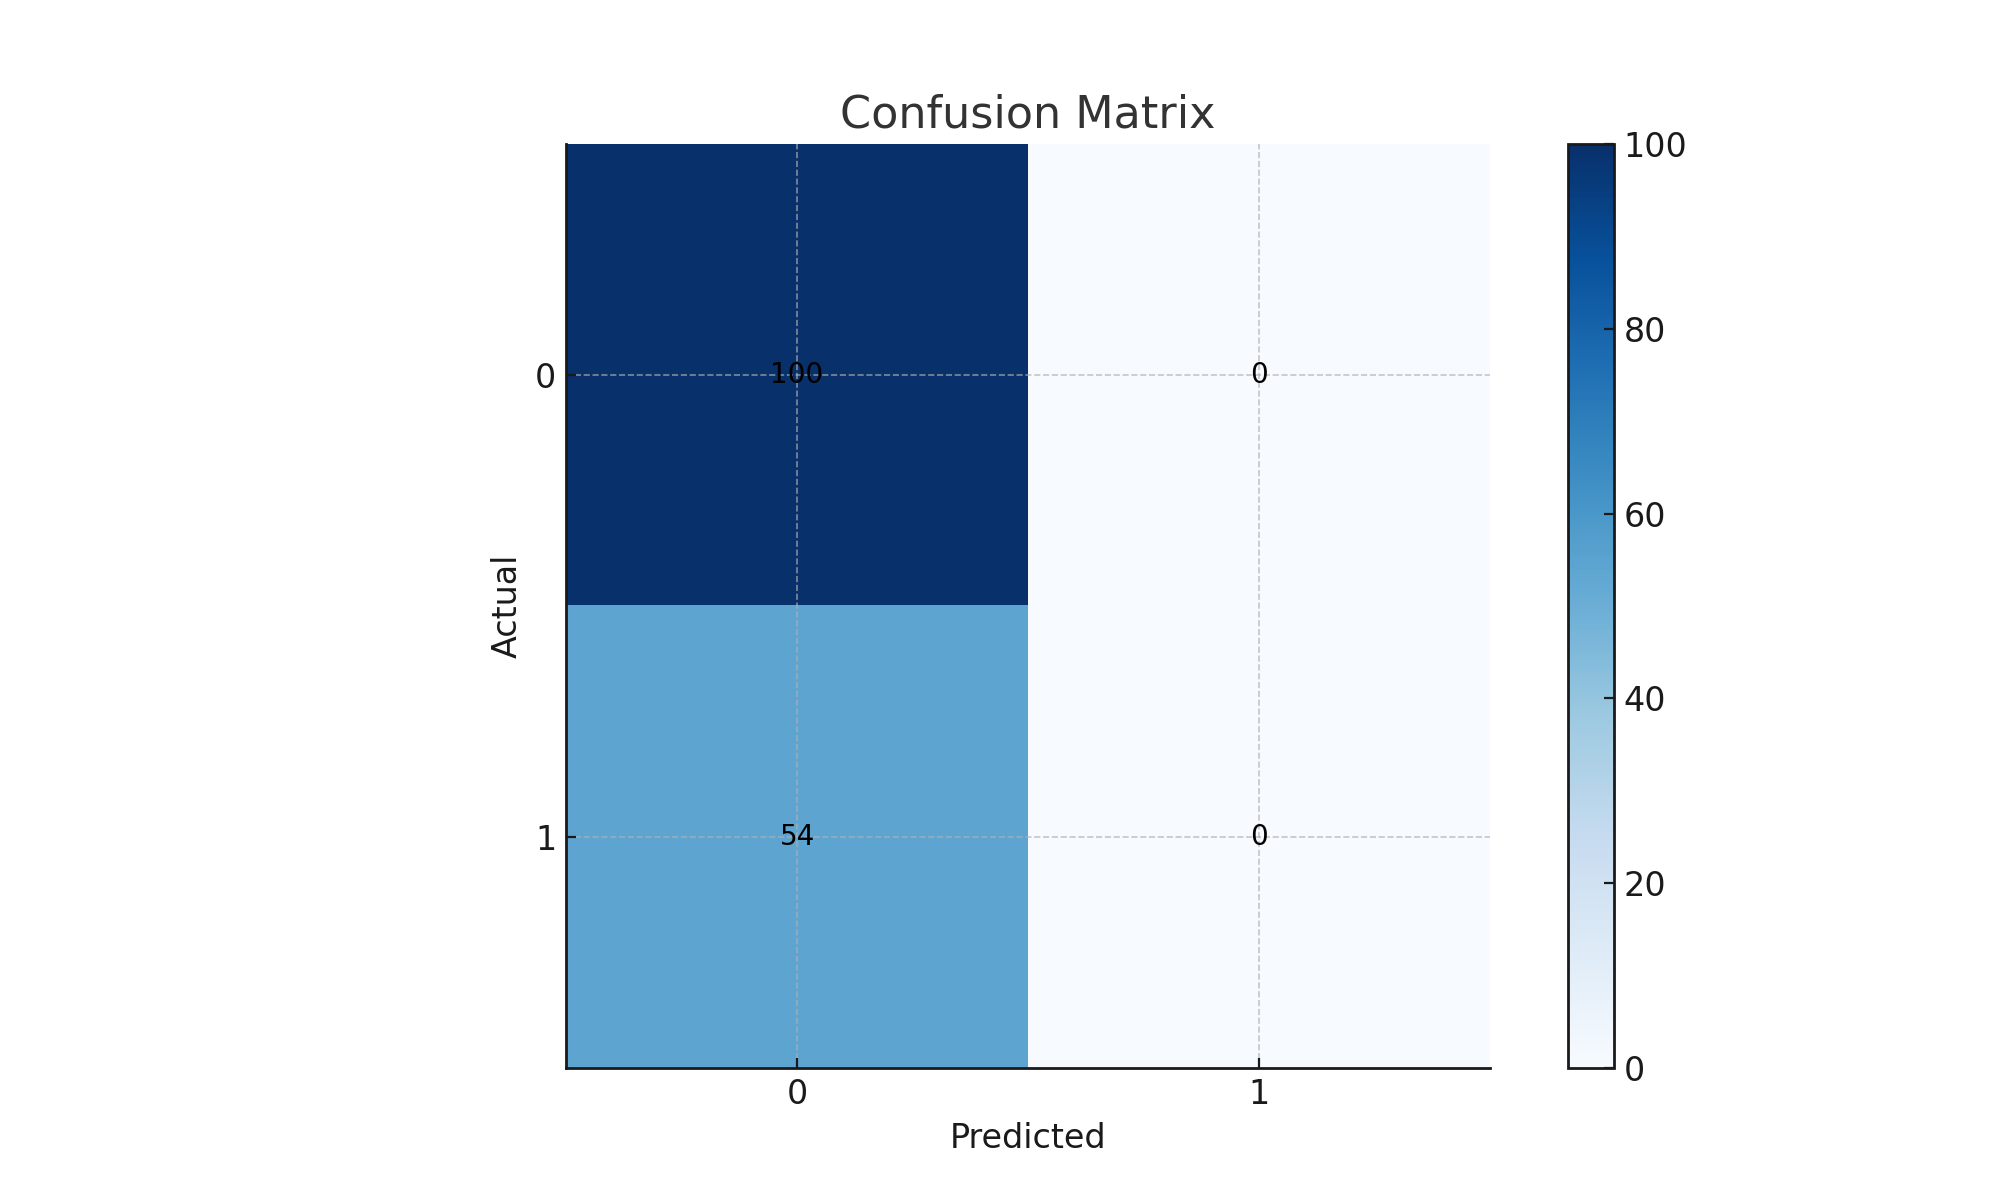
\includegraphics[width=0.85\linewidth]{confusion_matrix.png}
\caption{Confusion Matrix on Test Set}
\end{figure}

\subsection{Error Analysis}
The model performs well for class 0 (non-diabetic) but fails to predict class 1 due to imbalance in the dataset. Techniques such as class weighting or oversampling should be considered in future work.

\section{Discussion}
This implementation shows that a basic MLP without libraries can achieve reasonable performance. However, it also exposes limitations due to class imbalance and lack of regularization. Improvements could include:
\begin{itemize}
    \item L2 regularization
    \item Dropout layers
    \item Using more layers or neurons
    \item Implementing optimizers like Adam
\end{itemize}

\section{Conclusion and Future Work}
We have demonstrated the implementation of a multilayer perceptron from scratch in Python. The model performs adequately on a medical dataset, showcasing the potential of even simple neural networks. Future work could involve extending this approach to more complex models or integrating additional patient data for better prediction accuracy.

\section*{Code Repository}
All code and resources are available at: \url{https://github.com/Hibaamenhar/diabetes-mlp}

\section*{References}
\begin{itemize}
    \item UCI Pima Indians Diabetes Dataset: \url{https://www.kaggle.com/datasets/uciml/pima-indians-diabetes-database}
    \item Y. LeCun, Y. Bengio, and G. Hinton. "Deep learning." Nature 521.7553 (2015): 436–444.
    \item Goodfellow, Ian, et al. "Deep Learning." MIT Press (2016).
    \item Géron, Aurélien. "Hands-on Machine Learning with Scikit-Learn, Keras & TensorFlow." O’Reilly (2019).
\end{itemize}

\end{document}

